\section{Cell Growth}

% Task 2.1

% Simulate the growth of tumour cells for t=1200. Does the growth reach a steady state?
% If it has not, then experiment with the final time and determine the Time required to reach a steady state.

% 10 marks for basic simulation, 5 marks for showing time to reach final time 
% You can also use analytical methods to do the same

% Task 2.2

% Will the rate of growth reach a steady state or will the number increase as you keep increasing the size of the grid?
% What will happen if the value of M is changed - pick two values on either side of the value given.
% The issues associated with the numerical strategy you are employing,

% 5 marks for the part where you suggest what happens when the value of M changes, and why this is important

\[ \frac{dN}{dt}  = kNln\left(\frac{M}{n} \right) \]
\[ N = \dfrac{M}{10^{4e^{-kt}}}  \]

\clearpage

\begin{figure}[ht]
    \centering
    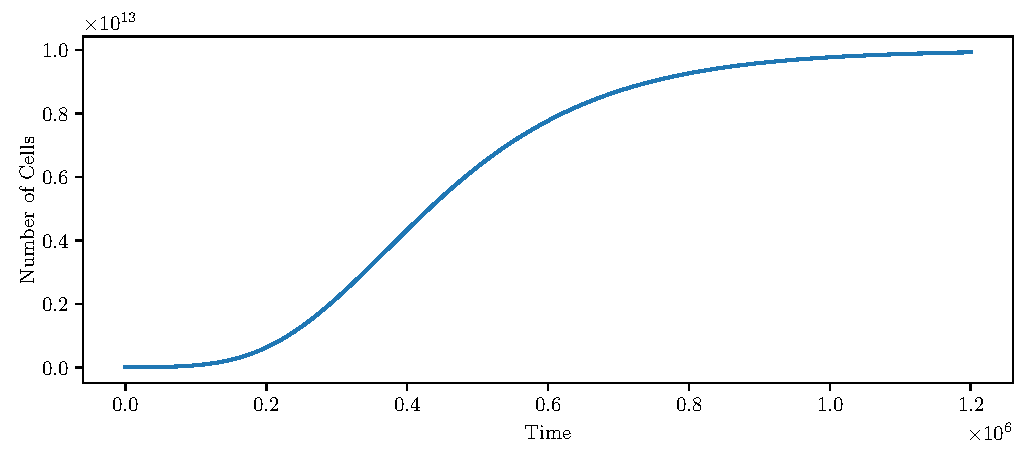
\includegraphics[width=14cm]{task2-1}
    \caption[Cell growth simulation]{Cell growth simulation}
    \label{fig:task2-1}
\end{figure}

\clearpage

\begin{figure}[ht]
    \centering
    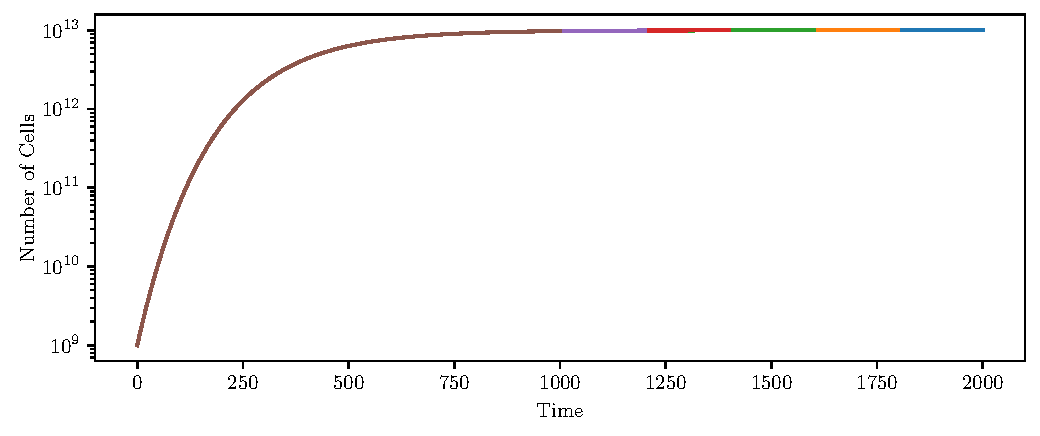
\includegraphics[width=14cm]{task2-1-t}
    \caption[Cell growth simulation with different T values]{Cell growth simulation with different T values}
    \label{fig:task2-1-t}
\end{figure}

\begin{center}
\begin{tabular}{c | c c} 
    T & Cells & \ Full \\
    \hline
    2000 & 1.00e+13 & 0.9999\% \\
    1800 & 1.00e+13 & 0.9998\% \\
    1600 & 9.99e+12 & 0.9994\% \\
    1400 & 9.98e+12 & 0.9979\% \\
    1200 & 9.93e+12 & 0.9931\% \\
    1000 & 9.77e+12 & 0.9774\% \\    
\end{tabular}
\end{center}

\clearpage

\begin{figure}[ht]
    \centering
    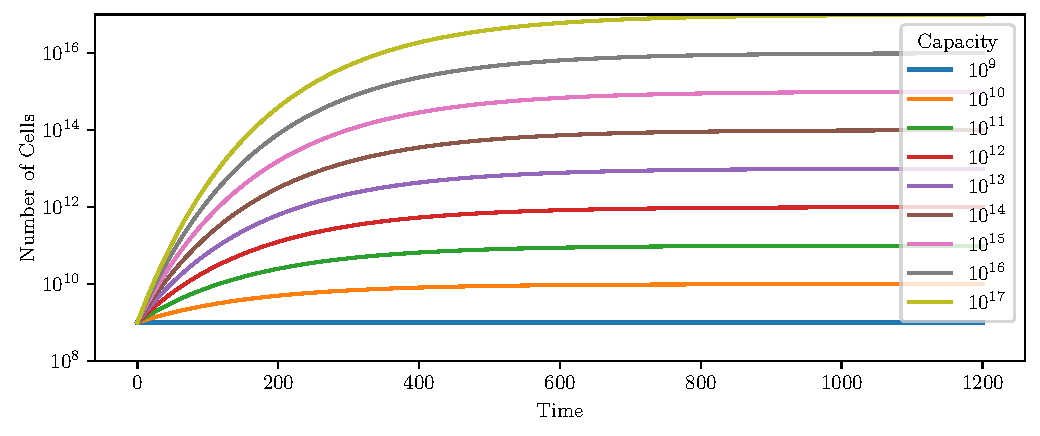
\includegraphics[width=14cm]{task2-1-m}
    \caption[Cell growth simulation with different capacity values]{Cell growth simulation with different capacity values}
    \label{fig:task2-1-m}
\end{figure}

\clearpage

\begin{figure}[ht]
    \centering
    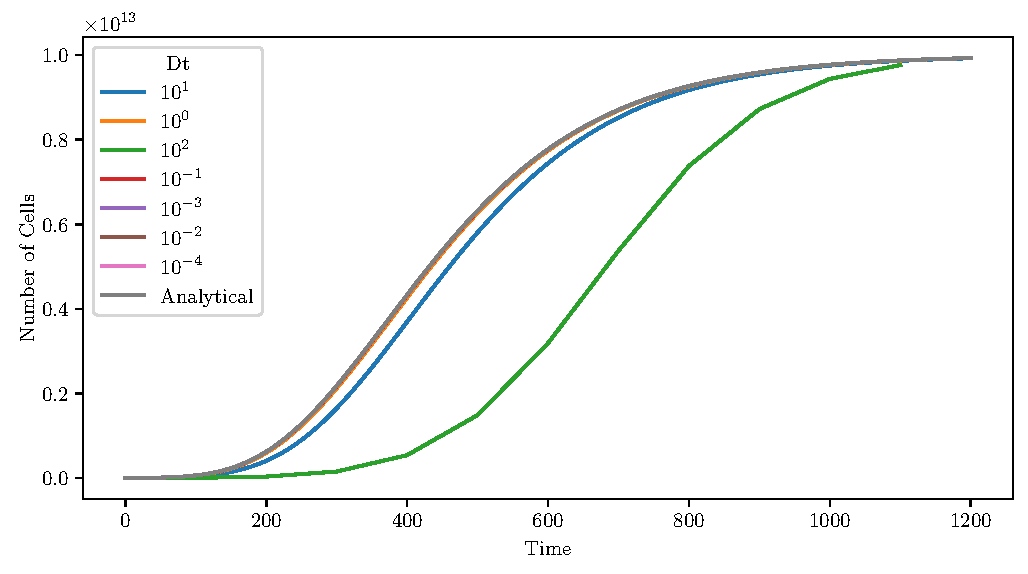
\includegraphics[width=14cm]{task2-1-h}
    \caption[Cell growth simulation with different dt values]{Cell growth simulation with different dt values}
    \label{fig:task2-1-h}
\end{figure}

\begin{figure}[ht]
    \centering
    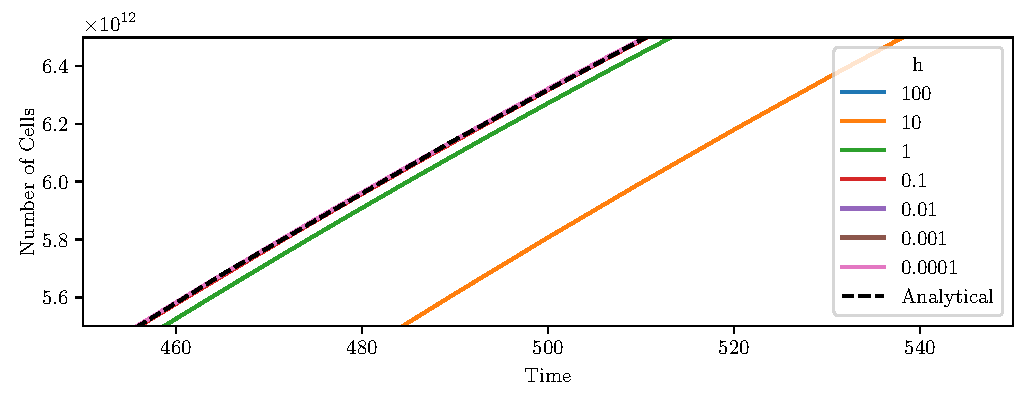
\includegraphics[width=14cm]{task2-1-h-zoom}
    \caption[Cell growth simulation with different dt values (zoomed)]{Cell growth simulation with different dt values (zoomed)}
    \label{fig:task2-1-h-zoom}
\end{figure}

\begin{center}
\begin{tabular}{c | c} 
    h & Error \\
    \hline
    100 & 66.69\% \\
    10 & 5.296\% \\
    1 & 0.5238\% \\
    0.1 & 0.05233\% \\
    0.01 & 0.005233\% \\
    0.001 & 0.0005239\% \\
    0.0001 & 5.82e-05\% \\
    Analytical & 0.0 \\
\end{tabular}
\end{center}

\clearpage

\begin{figure}[ht]
    \centering
    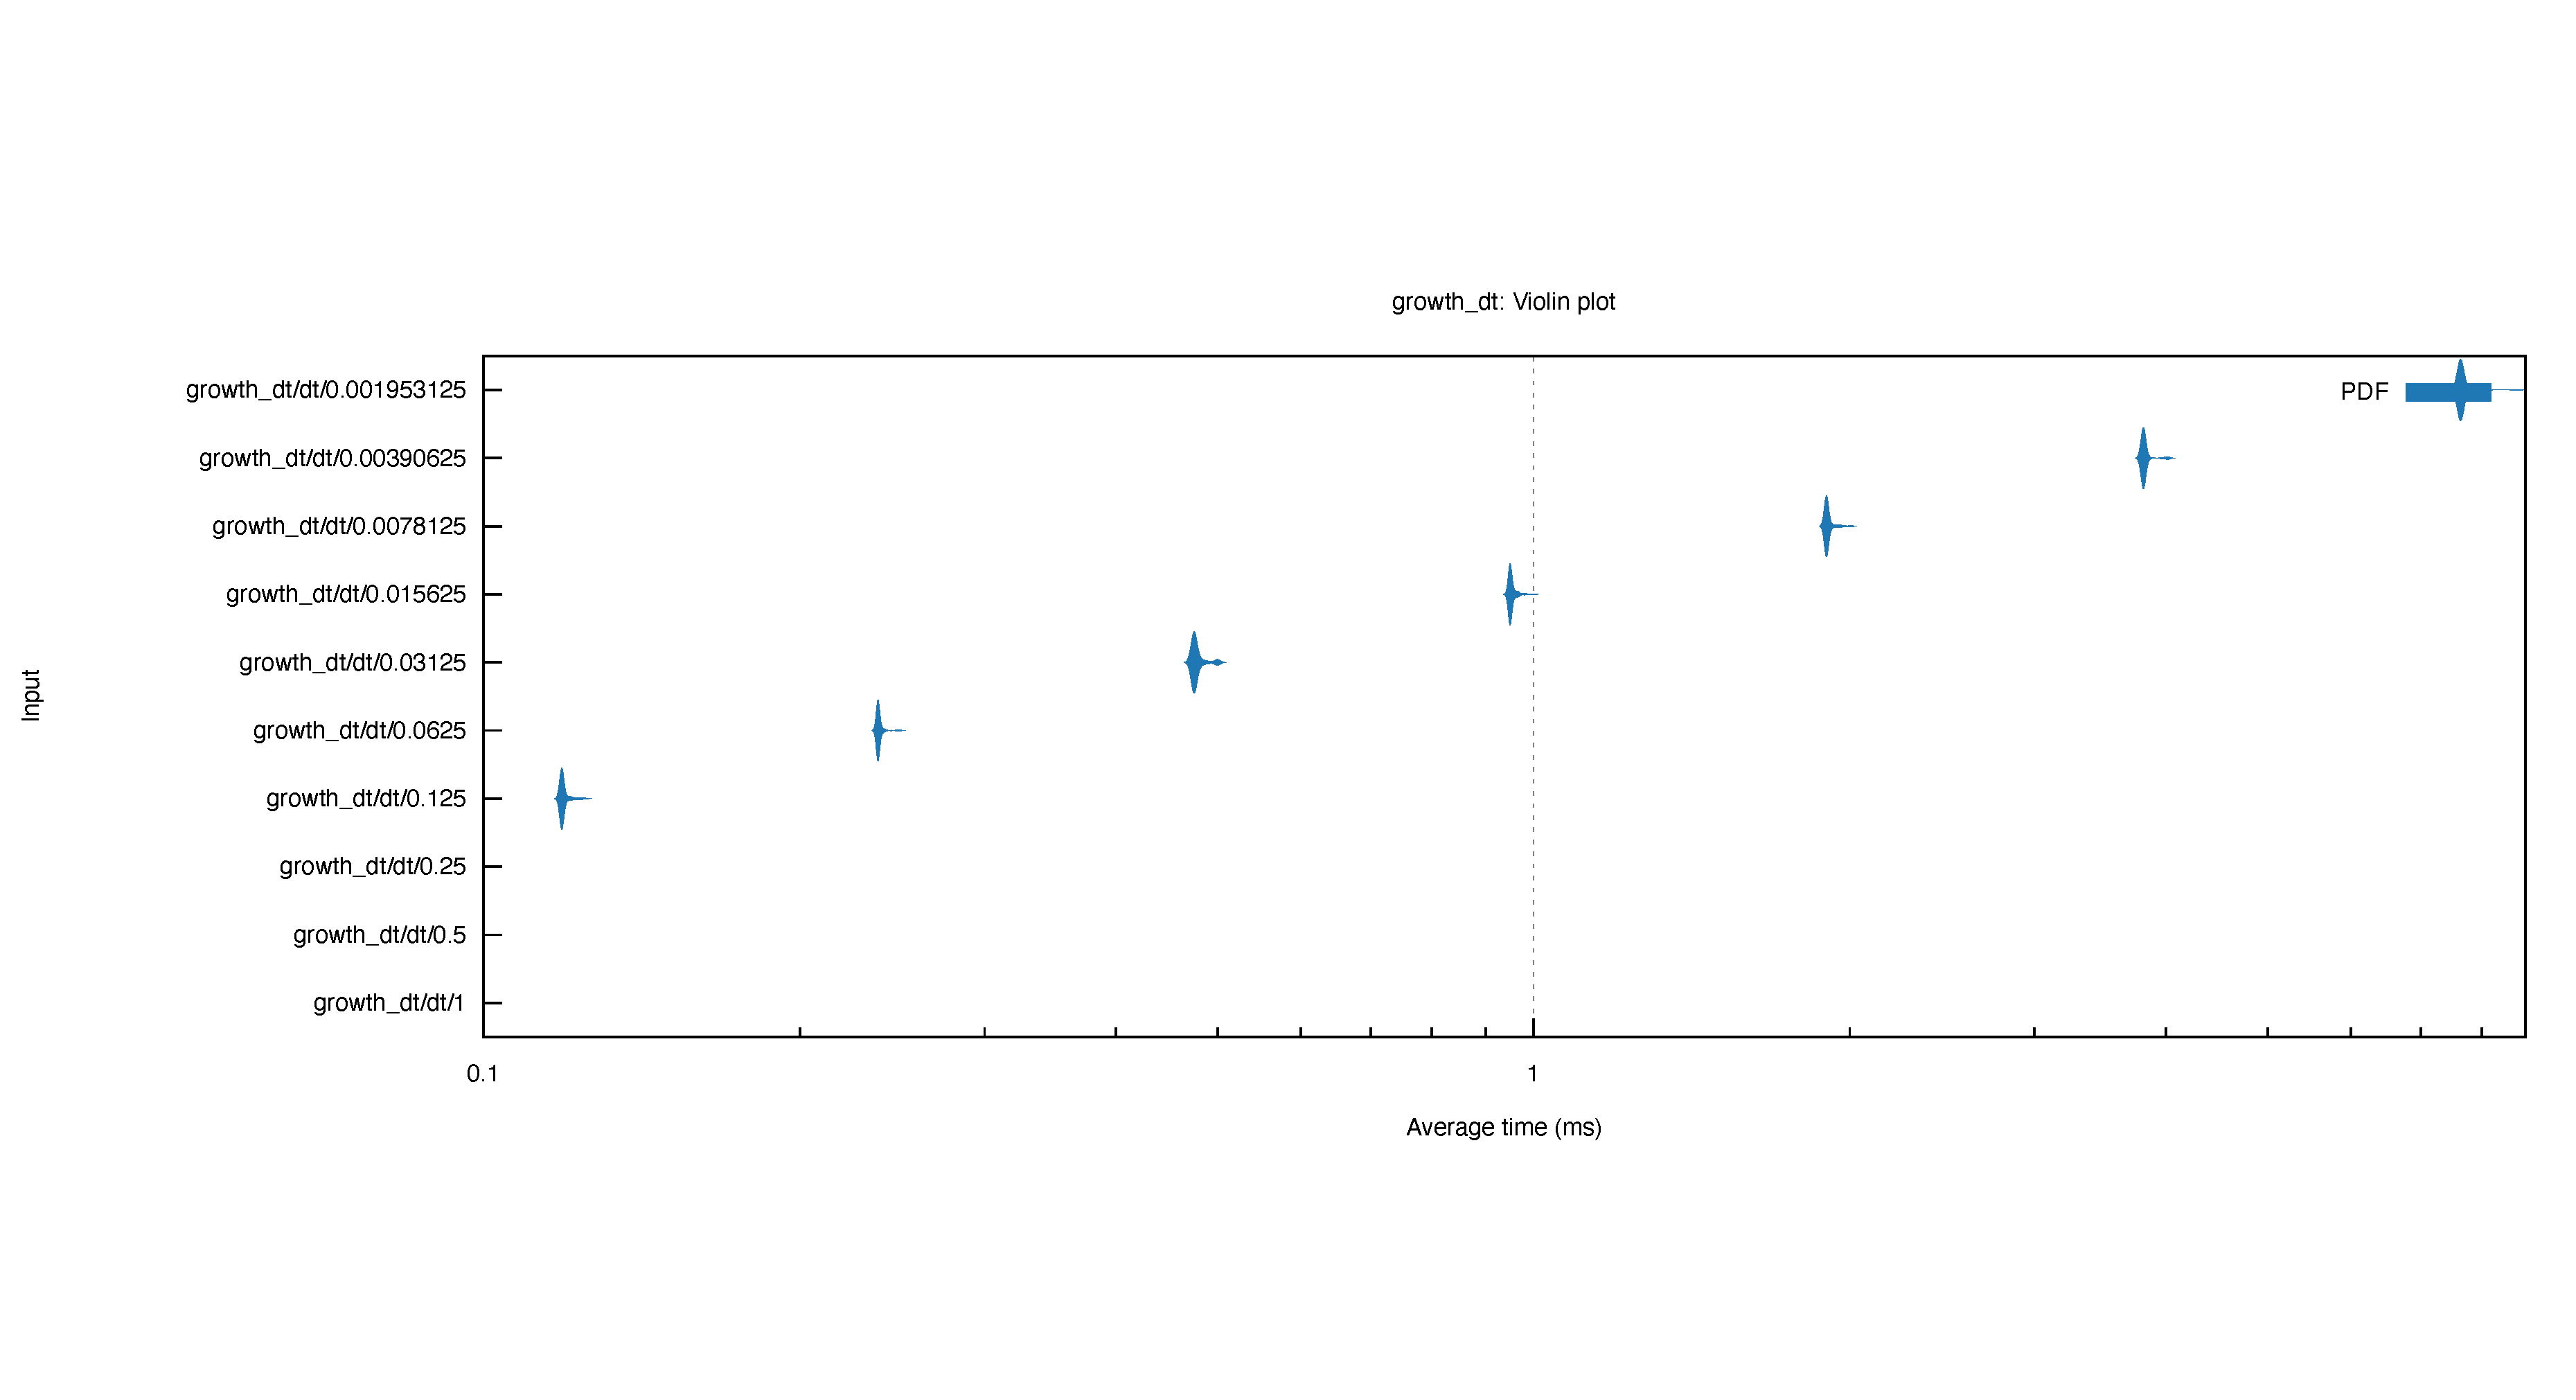
\includegraphics[width=14cm]{growth-dt-criterion}
    \caption[Cell growth criterion]{Cell growth criterion}
    \label{fig:growth-dt-criterion}
\end{figure}

\clearpage

\begin{figure}[ht]
    \centering
    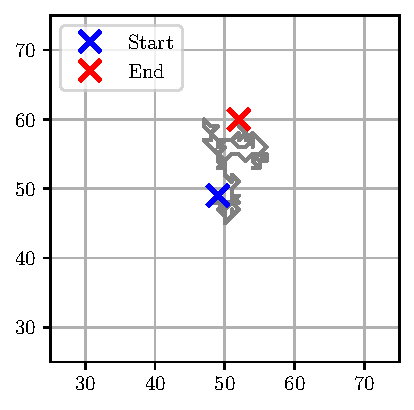
\includegraphics[width=5cm]{task2-2}
    \caption[Cell growth simulation with diagonal movement]{Cell growth simulation with diagonal movement}
    \label{fig:task2-2}
\end{figure}

\clearpage

\begin{figure}[ht]
    \centering
    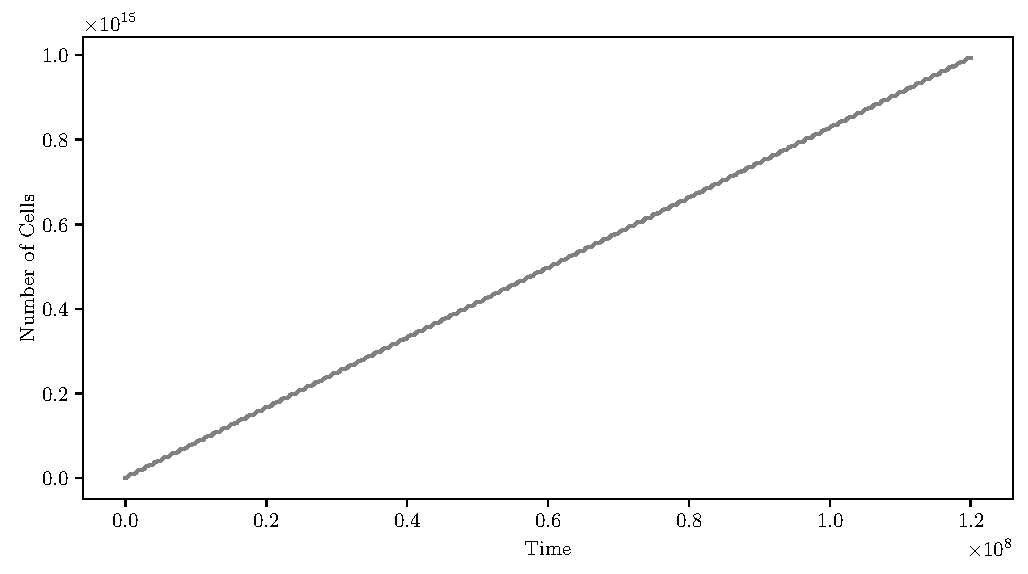
\includegraphics[width=14cm]{task2-2-total}
    \caption[Cell growth simulation with diagonal movement (total cells)]{Cell growth simulation with diagonal movement (total cells)}
    \label{fig:task2-2-total}
\end{figure}

\begin{figure}[ht]
    \centering
    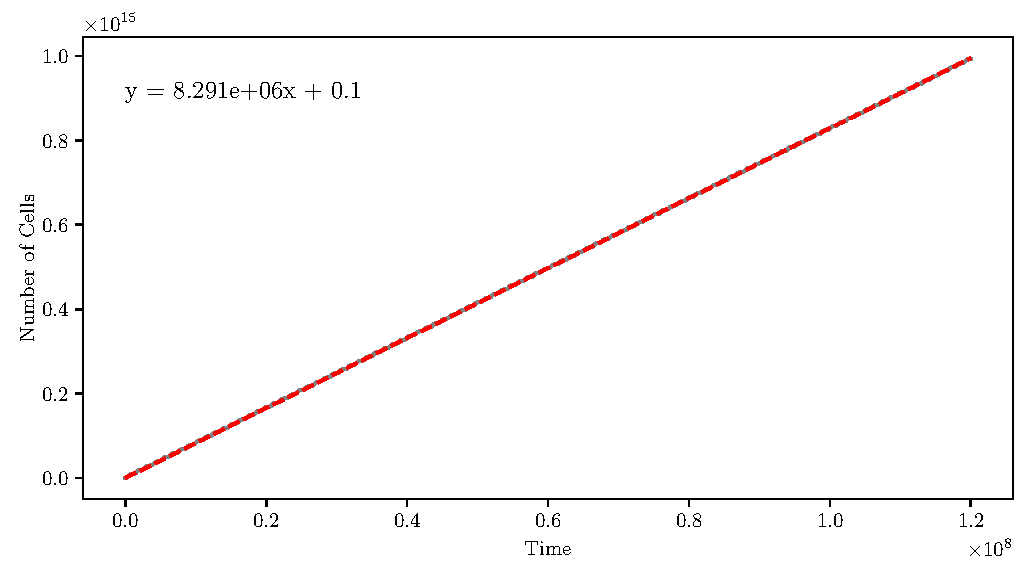
\includegraphics[width=14cm]{task2-2-total-linear}
    \caption[Cell growth simulation with diagonal movement (total cells) linear estimation]{Cell growth simulation with diagonal movement (total cells) linear estimation}
    \label{fig:task2-2-total-linear}
\end{figure}